\section{Auswertung}
\label{sec:auswertung}

\begin{figure}
    \centering
    \begin{tabular}{cc}
      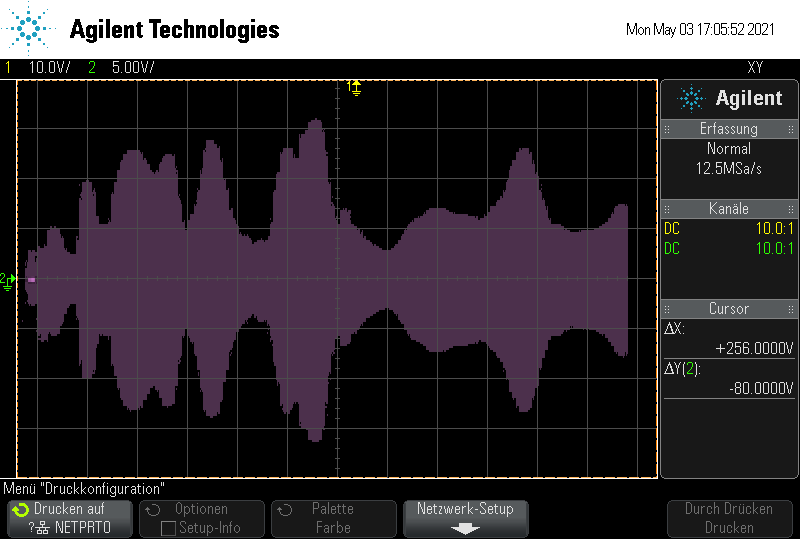
\includegraphics[width=65mm]{Daten/Zyinder/Zylinder_1.png} &   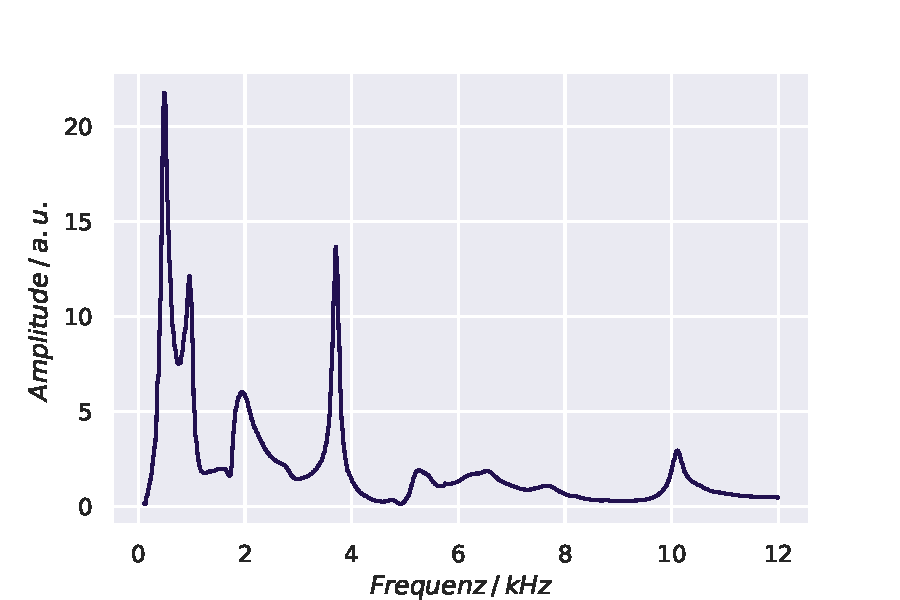
\includegraphics[width=65mm]{Daten/Zyinder/Zylinder_1.pdf} \\
    (a) 1 Zylinder & (b) 1 Zylinder \\[6pt]
     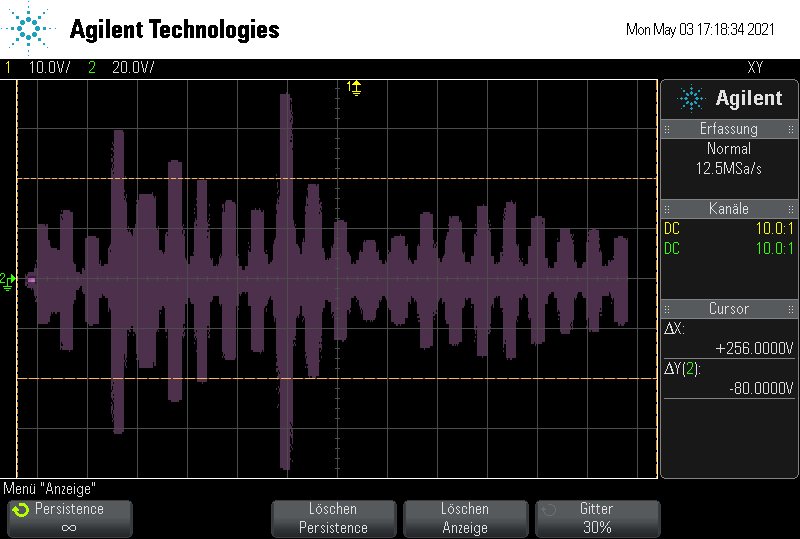
\includegraphics[width=65mm]{Daten/Zyinder/Zylinder_6.png} &   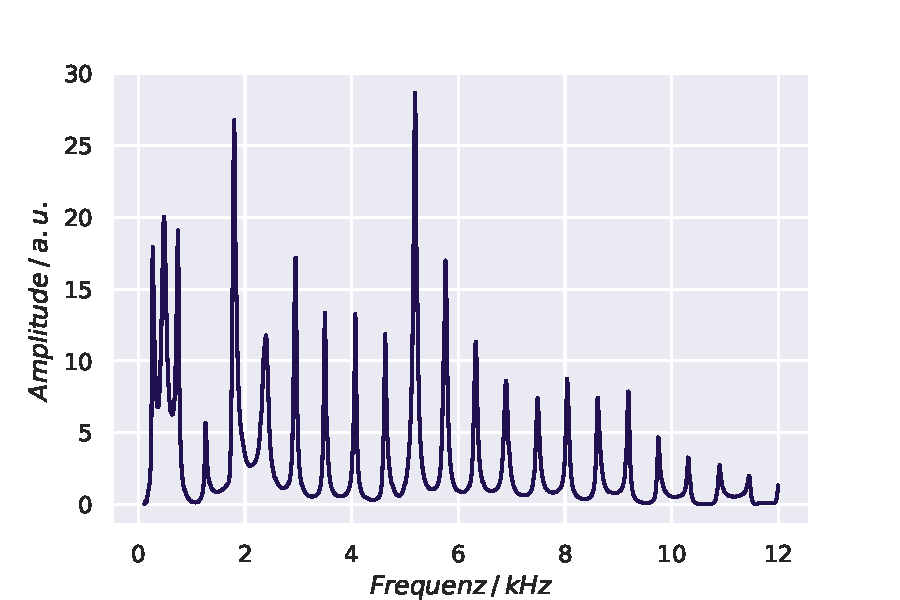
\includegraphics[width=65mm]{Daten/Zyinder/Zylinder_6.pdf} \\
    (c) 6 Zylinder & (d) 6 Zylinder \\[6pt]
    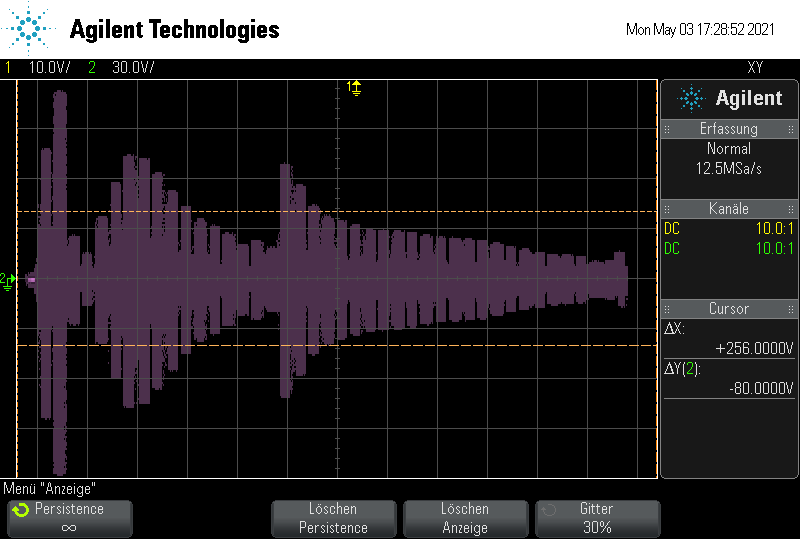
\includegraphics[width=65mm]{Daten/Zyinder/Zylinder_12.png} &   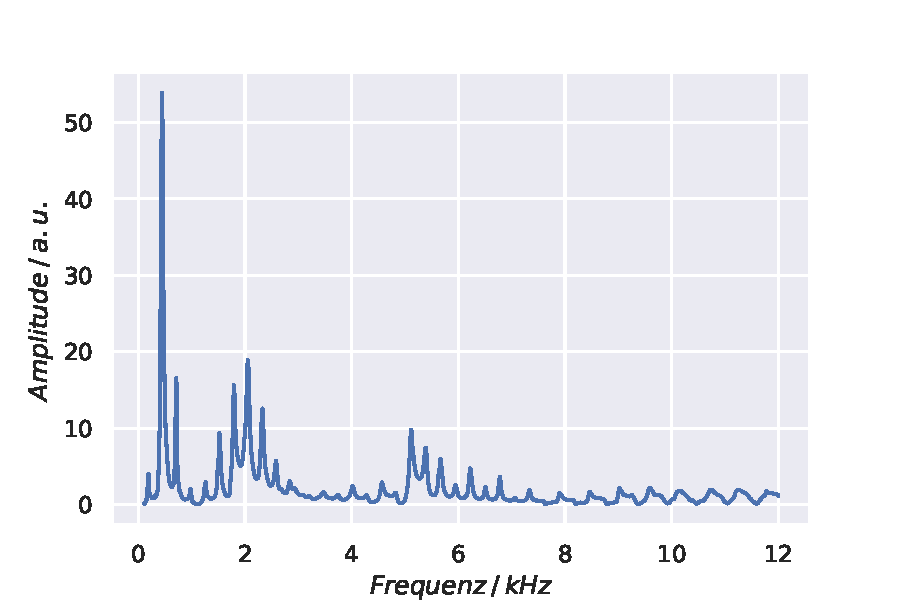
\includegraphics[width=65mm]{Daten/Zyinder/Zylinder_12.pdf} \\
    (c) 12 Zylinder & (d) 12 Zylinder \\[6pt]
    \end{tabular}
    \caption{Gemessene Frequenzspektren der Zylinder-Resonatoren mit unterschiedlicher Länge. Die Messung am Oszillator ist links angegeben und die Messung am Computer rechts. } 
    \label{fig:zyl1-6-12}
\end{figure}

\begin{figure}
    \centering
    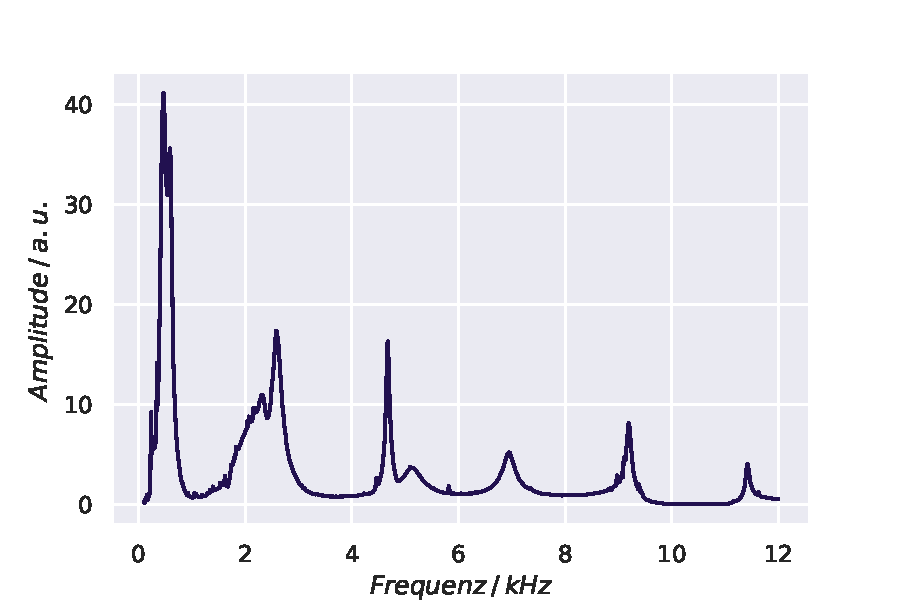
\includegraphics[width=0.8\textwidth]{Daten/Festkörper/FK_75mm.pdf}
    \caption{Das Frequenzspektrum eines $75 \,\si{\milli\metre}$ langen Zylinder-Resonators. }
    \label{fig:fkp75mm}
\end{figure}

\begin{figure}
    \centering
    \begin{tabular}{c}
    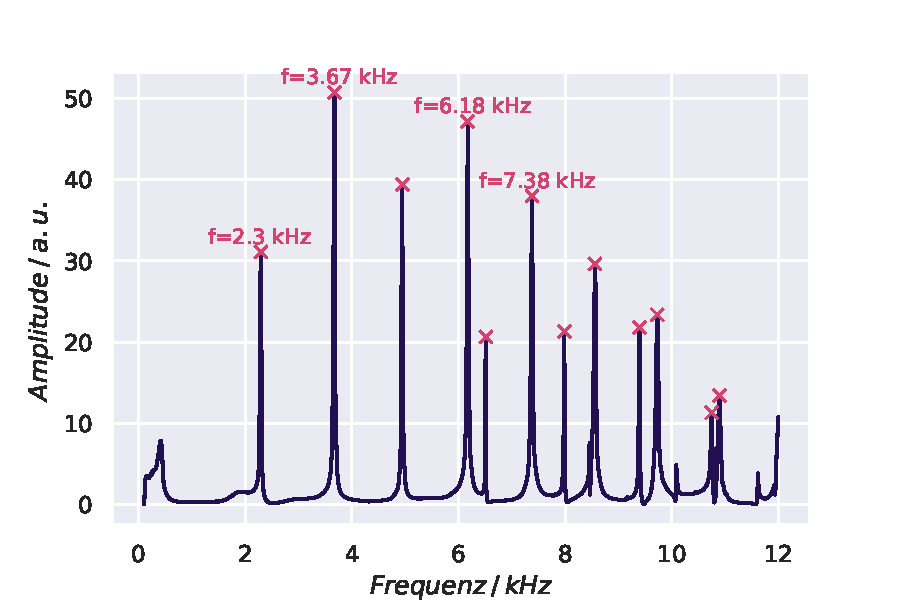
\includegraphics[width=0.6\textwidth]{Daten/Wasserstoff/H_180.pdf} \\
    (a) Messung am Computer \\[6pt]
    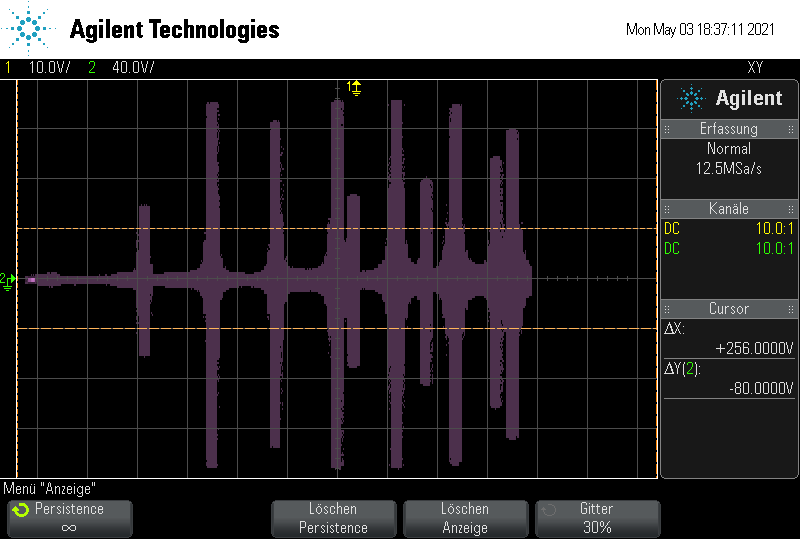
\includegraphics[width=0.6\textwidth]{Daten/Wasserstoff/H_180.png} \\
    (b) Messung am Oszilloskop \\[6pt]
    \end{tabular}
    \caption{Das Frequenzspektrum eines kugelförmigen Hohlraumresonators bei einer Ausrichtung von $\theta = 180\si{°}$ in dem Bereich $0.1 \,\si{\kilo\hertz}$ bis $10 \,\si{\kilo\hertz}$. }
    \label{fig:h180}
\end{figure}


\begin{figure}
    \centering
    \begin{tabular}{cc}
      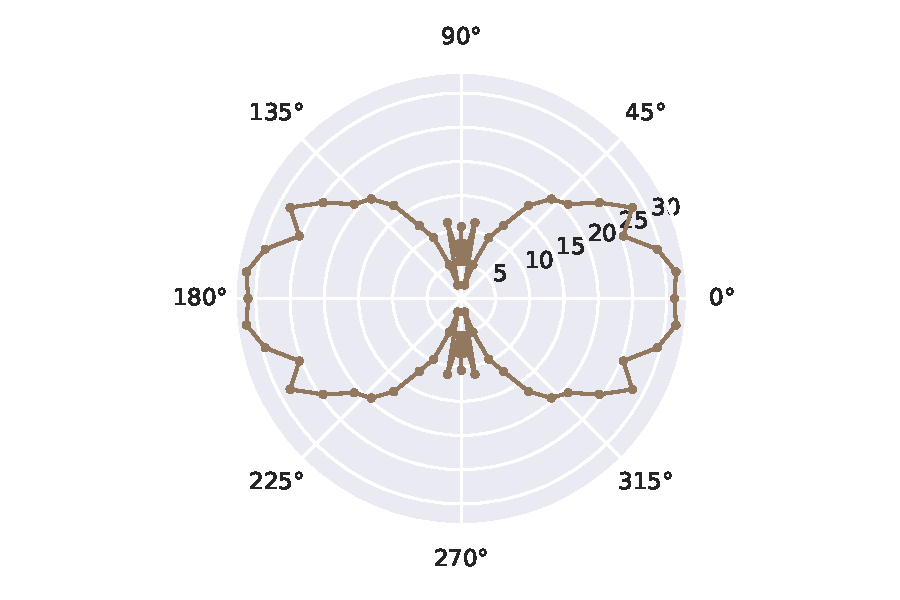
\includegraphics[width=65mm]{Daten/Wasserstoff/peak0.pdf} &   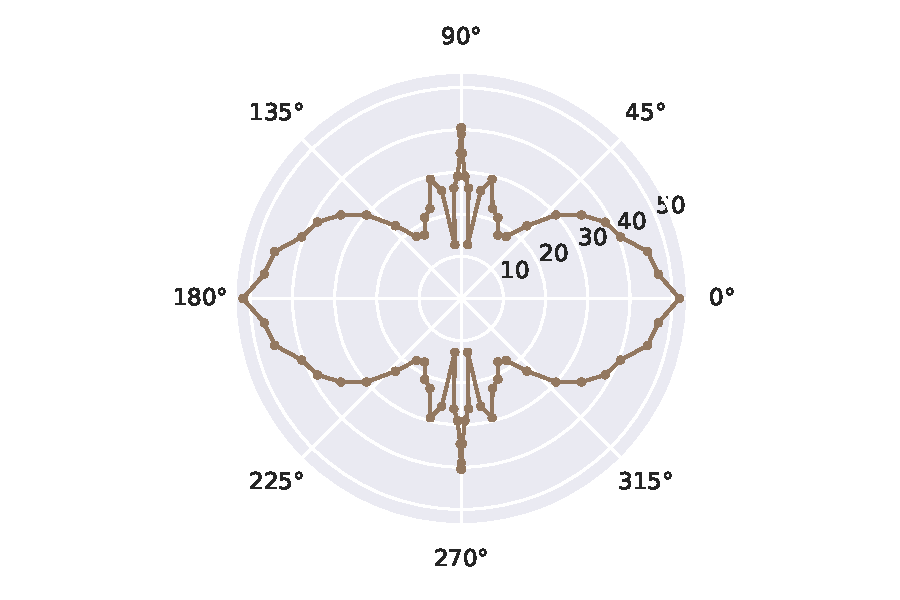
\includegraphics[width=65mm]{Daten/Wasserstoff/peak1.pdf} \\
    (a) Resonanz bei $2.3 \,\si{\kilo\hertz} $& (b) Resonanz bei $3.67 \,\si{\kilo\hertz}$ \\[6pt]
    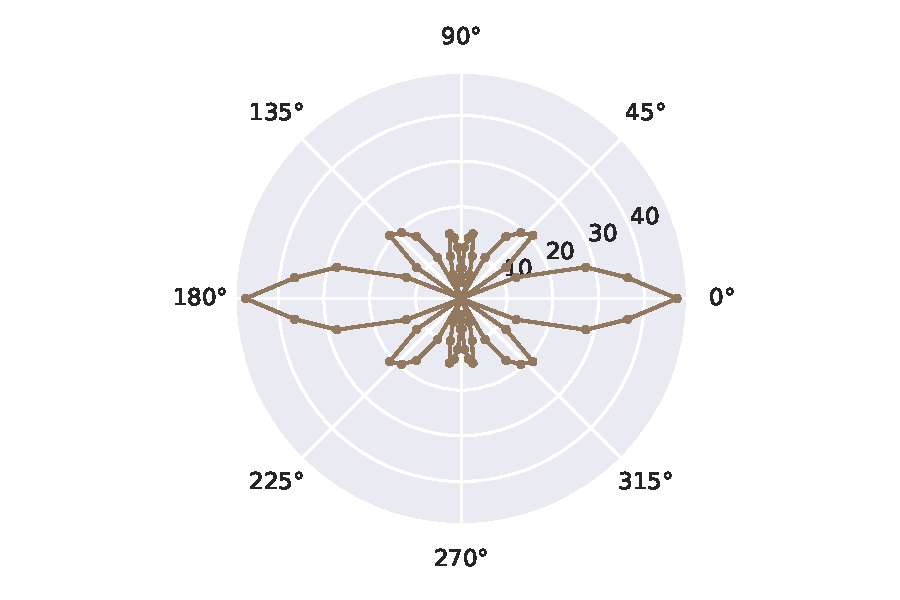
\includegraphics[width=65mm]{Daten/Wasserstoff/peak2.pdf} &   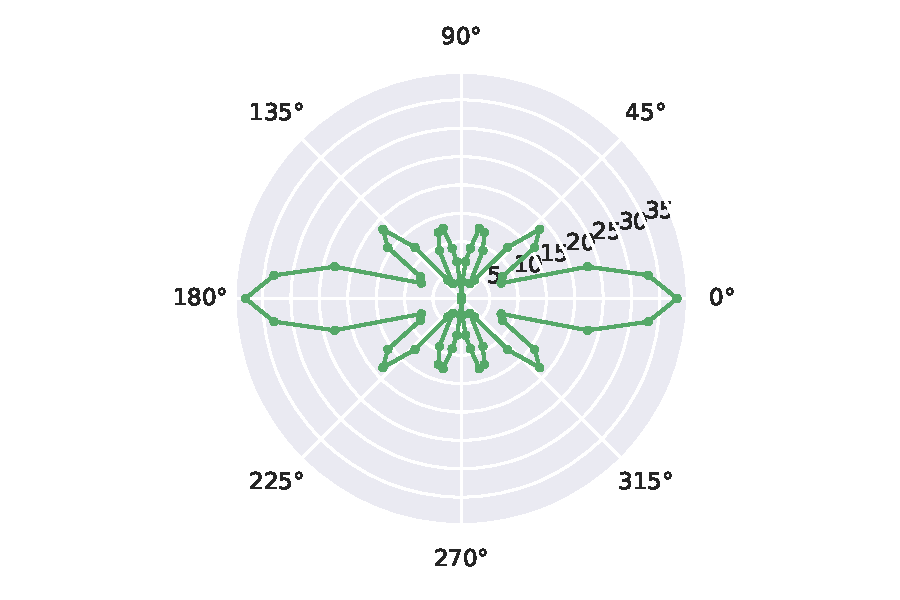
\includegraphics[width=65mm]{Daten/Wasserstoff/peak3.pdf} \\
    (c) Resonanz bei $6.18 \,\si{\kilo\hertz}$ & (d) Resonanz bei $7.38 \,\si{\kilo\hertz}$ \\[6pt]
    \end{tabular}
    \caption{Amplitudenmessung an den Resonanzfrequenzen in Abhängigkeit vom Azimutwinkel $\phi$. } 
    \label{fig:hpeaks}
\end{figure}